\section{Diseño}

\subsection{Diseño del \textit{pulser}}

\subsubsection{SRD como afilador de flanco}

En la sección \textcolor{red}{AGREGAR REF\ref{TODO}} fue explicado como un diodo
\textit{SRD} funciona como afilador de flanco.

En la figura \ref{fig:srd_sharpener} puede observarse un circuito que demuestra
el funcionamiento.

\begin{figure}
  \centering
    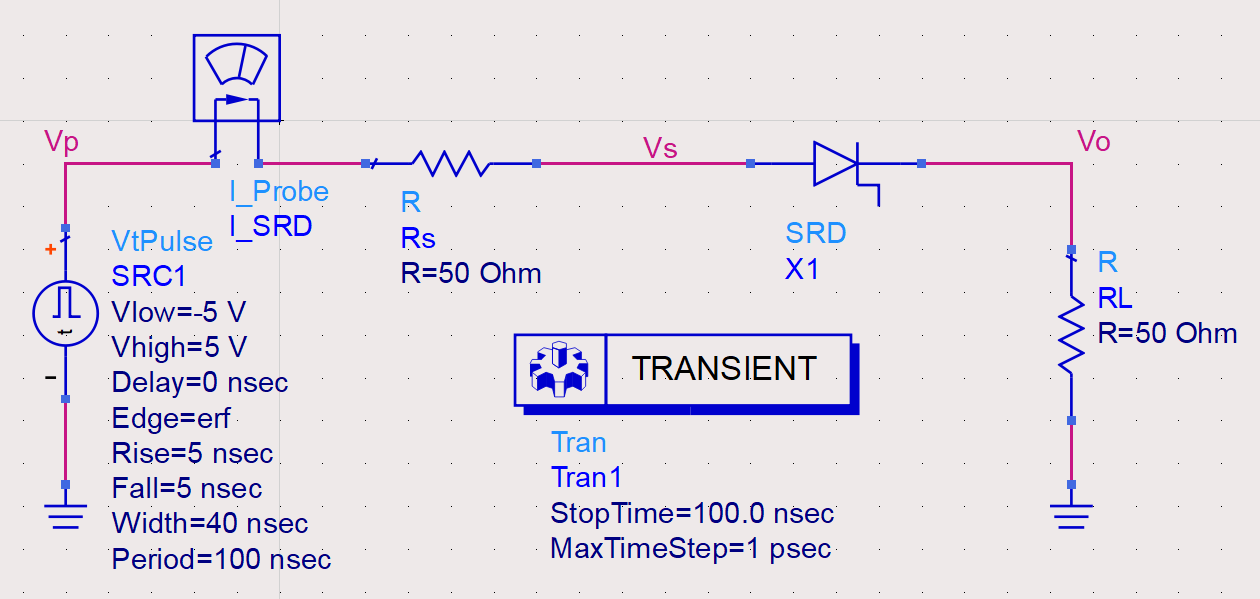
\includegraphics[width=0.6\textwidth]{images/srd_sharpener_circuit.png}
    \caption{Circuito afilador de flanco con SRD}
    \label{fig:srd_sharpener}
\end{figure}

\begin{figure}[tbp]
    \centering
    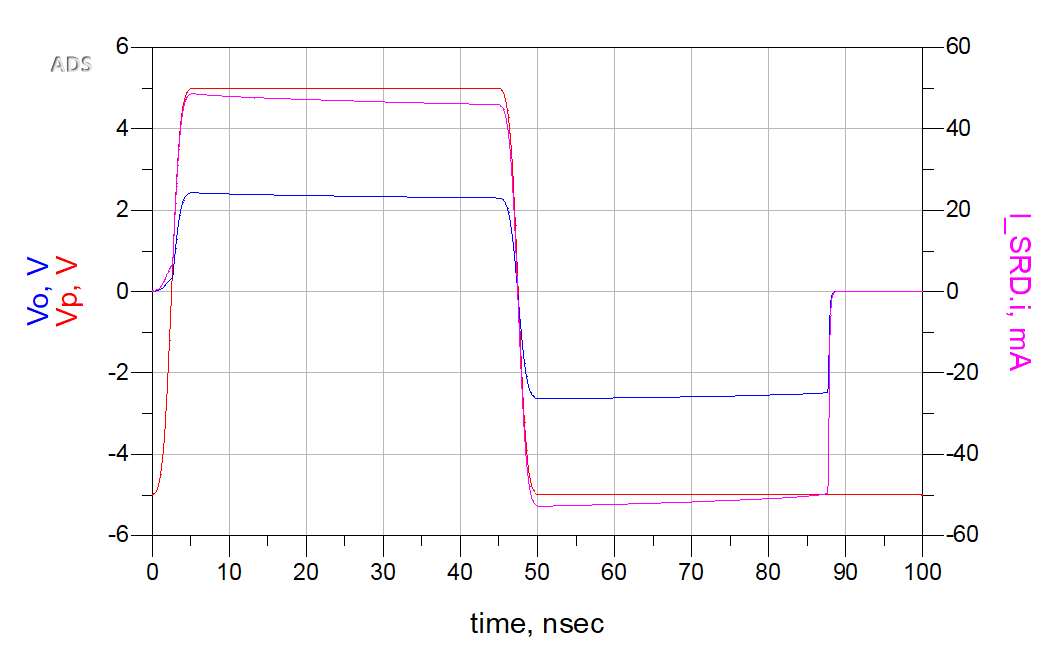
\includegraphics[width=0.8\textwidth]{images/srd_sharpener_result.png}
    \caption{Resultado de simulación.}
    \label{fig:srd_sharpener_result}
\end{figure}

\begin{figure}[tbp]
    \centering
    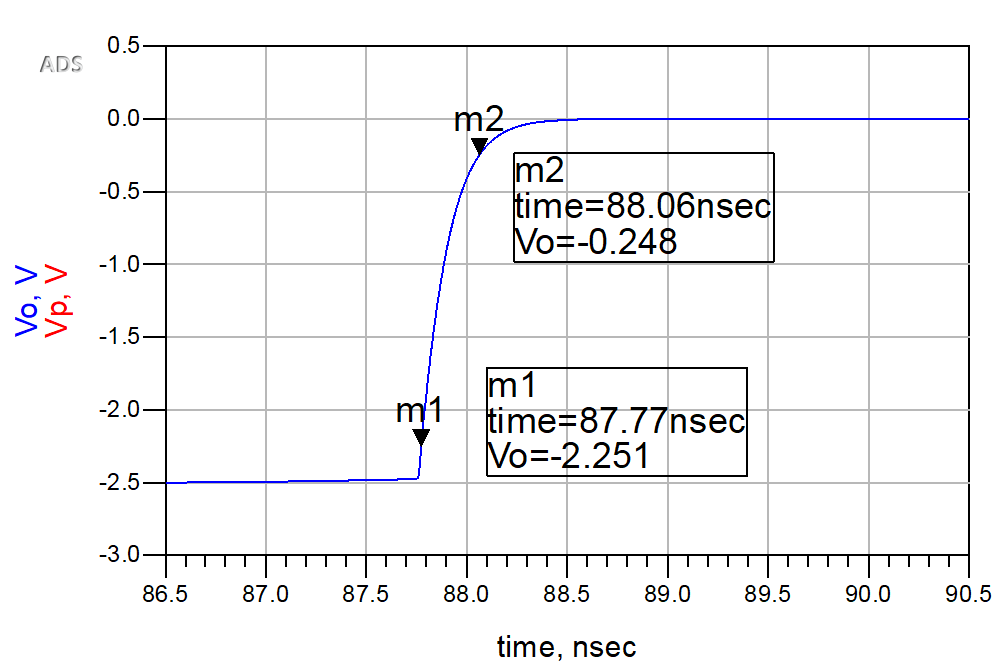
\includegraphics[width=0.8\textwidth]{images/srd_sharpener_result_rise_time.png}
    \caption{Tiempo de crecimiento.}
    \label{fig:srd_sharpener_result_rise_time}
\end{figure}

El circuito está compuesto por un generador de cuadrada lento, con tiempos de
crecimiento y decrecimiento de \qty{5}{\nano\second}, en serie una resistencia
de fuente $R_s$ de valor \qty{50}{\ohm}. La carga del circuito es la resistencia
$R_L$ de \qty{50}{\ohm}.

En la figura \ref{fig:srd_sharpener_result} se observa el resultado de la
simulación. Vemos que, hasta aproximadamente \qty{85}{\nano\second}, la señal de
salida $V_o$ es igual a la señal de entrada, afectada por el divisor entre $R_L$
y $R_s$, $\frac{R_L}7{R_L+R_s}$. Durante este tiempo, el \textit{SRD} presenta
una baja impedancia. En la porción positiva de la señal de entrada $V_p$, esto
es coincidente con un diodo usual, ya que el mismo se encuentra polarizado en
directa. En lo que destaca el \textit{SRD} de un diodo usual, es que luego de que la
tensión de entrada se invierta, este sigue presentando una baja impedancia. Esto
se debe al gran tiempo de vida de sus portadores minoritarios, lo que requiere
un tiempo apreciable para descargarlos y pasar al estado de alta impedancia.

Se observa en la forma de onda de $V_o$ que esta transición se da alrededor de
\qty{85}{\nano\second}, done la tensión de salida cae abruptamente a $0$. En la
figura \ref{fig:srd_sharpener_result} puede observarse el comportamiento
de la corriente. Se observa la misma caída abrupta en los
\qty{85}{\nano\second}, y una inversión en el signo de la corriente con la
inversión en el signo de la cuadrada de entrada.

Llamaremos corriente de inyección de carga $I_F$ a la corriente que circula por
el \textit{SRD} con sentido positivo. Esta corriente determina la carga
almacenada en el mismo, y ambas se relacionan mediante \cite{an918},
\cite{moll1969}

\begin{equation}
    Q_F = I_F \cdot \tau \cdot \left( 1 - e^{-t_F/\tau}\right)
\end{equation}

Para el circuito presentado, la corriente $I_F$ estará dada por

\begin{equation}
    I_{F} = \frac{V_h}{R_s+R_L}
\end{equation}

con $V_h$ el valor de la tensión positiva de la señal cuadrada de entrada.

Para la corriente de extracción de carga $I_R$, que es la corriente que extrae
carga durante el tiempo en el que el \textit{SRD} se encuentra en un estado de
baja impedancia y la corriente que circula es negativa, tenemos la siguiente
expresión

\begin{equation}
    I_{R} = \frac{V_l}{R_s+R_L}
\end{equation}

con $V_l$ el valor de la tensión negativa de la señal cuadrada de entrada.

En la figura \ref{fig:srd_sharpener_result_rise_time}, puede observarse el
tiempo de crecimiento del escalón generado con el apagado del \textit{SRD}. Se
toma el tiempo de crecimiento \qty{10}{\percent}-\qty{90}{\percent}. Siendo que
el escalón de tensión se da entre \qty{-2.5}{\volt} y \qty{0}{\volt}, tenemos
que el punto de \qty{10}{\percent} es $V_{10\%} = -2.5 \ V \ \cdot 0.9 =  2.25 \
V$, y el de \qty{90}{\percent} es $V_{90\%} = -2.5 \ V \ \cdot 0.1 =  -0.25 \
V$.

En cuanto a la magnitud del salto de tensión $\Delta V$, estará dado por el
valor de la tensión en el cátodo del \textit{SRD} antes de que pase al estado de
alta impedancia. Esta tensión estará dada por el divisor entre $R_L$ y $R_s$,

\begin{equation}
    \Delta V = V_l \cdot \frac{R_L}{R_L+R_s}
\end{equation}

Vemos por los marcadores de la figura, que estos tiempos son
\qty{87.77}{\nano\second} y \qty{88.06}{\nano\second} respectivamente, por lo
que tenemos un tiempo de crecimiento

\begin{equation}
    t_r = \qty{87.77}{\nano\second} - \qty{88.06}{\nano\second} =
    \qty{290}{\pico\second}
\end{equation}

Como fuese explicado en la sección \textcolor{red}{AGREGAR REF\ref{TODO}}, este
tiempo de crecimiento estará dado por el tiempo de transición del diodo y por el
tiempo del RC formado entre la capacidad de reversa del diodo y la resistencia
vista desde los nodos del capacitor.

\subsubsection{Generador de pulsos con \textit{stub}}

\paragraph{Principios del \textit{stub}}

Un \textit{stub} consiste de una línea de transmsión conectada en paralelo al
camino de la señal. Su efecto sobre la señal dependerá de su impedancia
característica, largo e impedancia de terminación \cite{pozar2011}.

Cuando el \textit{stub} se encuentra abierto, es decir, terminado por una
impedancia infinita, la señal propagada se verá reflejada con signo positivo, y
en el caso de una línea de transmisión sin pérdidas, con un factor de ganancia
unitario. En el caso de una línea de transmisión real, las pérdidas resultaran
en un factor de atenuación. \textcolor{red}{chequear esto de la atenuación, y lo
q sigue de las aplicaciones de un stub abierto}.  Este efecto permite generar
resonancias en ciertas frecuencias, útiles para filtrado de señales o adaptación
de impedancias.

En el caso de un \textit{stub} cortocircuitado, es decir, con una impedancia de
terminación igual a $0$, el efecto será una reflexión de la señal con fase
opuesta, y un factor de atenuación dado por las pérdidas de la línea.

El caso de interés para el circuito generador de pulsos, es el del \textit{stub}
cortocircuitado, ya que la reflexión de señal con fase opuesta, permite generar
un pulso en base a una forma de onda creciente o decreciente.

\begin{figure}[tbp]
    \centering
    
\includegraphics[width=0.8\textwidth]{images/placeholder.jpg}
    \caption{Reflexiones en un \textit{stub} cortocircuitado.}
    \label{fig:images-placeholder-jpg}
\end{figure}

En la figura \ref{TODO figura con funcionamiento temporal del stub} se observa
el principio de funcionamiento. Se observa un pulso de entrada, formado por una
forma de onda de tipo escalón, en nuestro caso este escalón será el mismo que en
la figura \ref{srd_sharpener_result_rise_time}. Este escalón se ve reflejado con
polaridad opuesta, y se suma al escalón de entrada.

Dado el tiempo de propagación de la línea de transmisión $T$, vemos que el
tiempo que tarda el pulso de entrada en reflejarse es $2*T$, el tiempo de un
camino de ida y vuelta. Dado que el pulso se forma cuando vuelve la componente
reflejada, vemos que el ancho de pulso estará dado por $2*T$. De esta forma, la
duración temporal del pulso y, por lo tanto, el ancho de banda del sistema,
estará dado por la longitud $L$ del \textit{stub}.

Desarrollar la expresión de $T$.


\paragraph{Generador de pulsos propuesto}

Un \textit{stub} es una línea de transmisión puesta a tierra en paralelo con la
señal. Una línea de transmisión puesta a tierra presenta una reflexión total de
la señal transmitida, con polaridad opuesta \cite{pozar2011}.

Agregando un \textit{stub} al afilador de pulsos descripto anteriormente, es
posible formar un pulso con el flanco rápido generado por el SRD.

El \textit{stub} actúa como una puesta a tierra para señales cuya variación temporal es
mucho más lenta que el tiempo de propagación en el mismo. Para el flanco
generado por el \textit{SRD}, la reflexión del mismo genera un pulso. El ancho
de este pulso es el doble del retardo temporal del \textit{stub}

\begin{equation}
    T_{pulso} = 2 \cdot T_{stub}
\end{equation}

\begin{figure}[tbp]
    \centering
    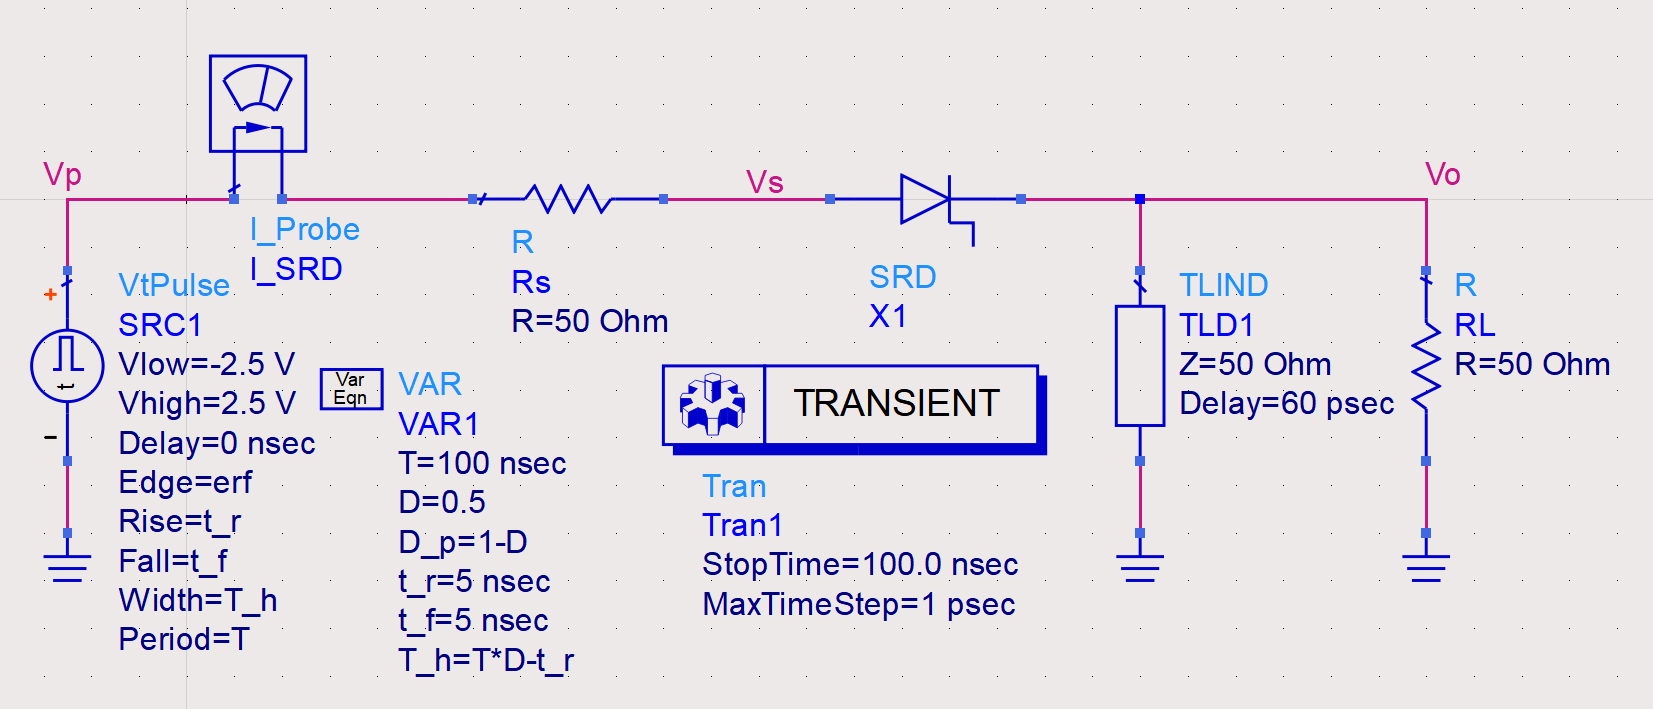
\includegraphics[width=0.8\textwidth]{images/stub_generator_circuit.png}
    \caption{Generador de pulsos basado en \textit{stub}}
    \label{fig:stub_generator_circuit}
\end{figure}

\begin{figure}[tbp]
    \centering
    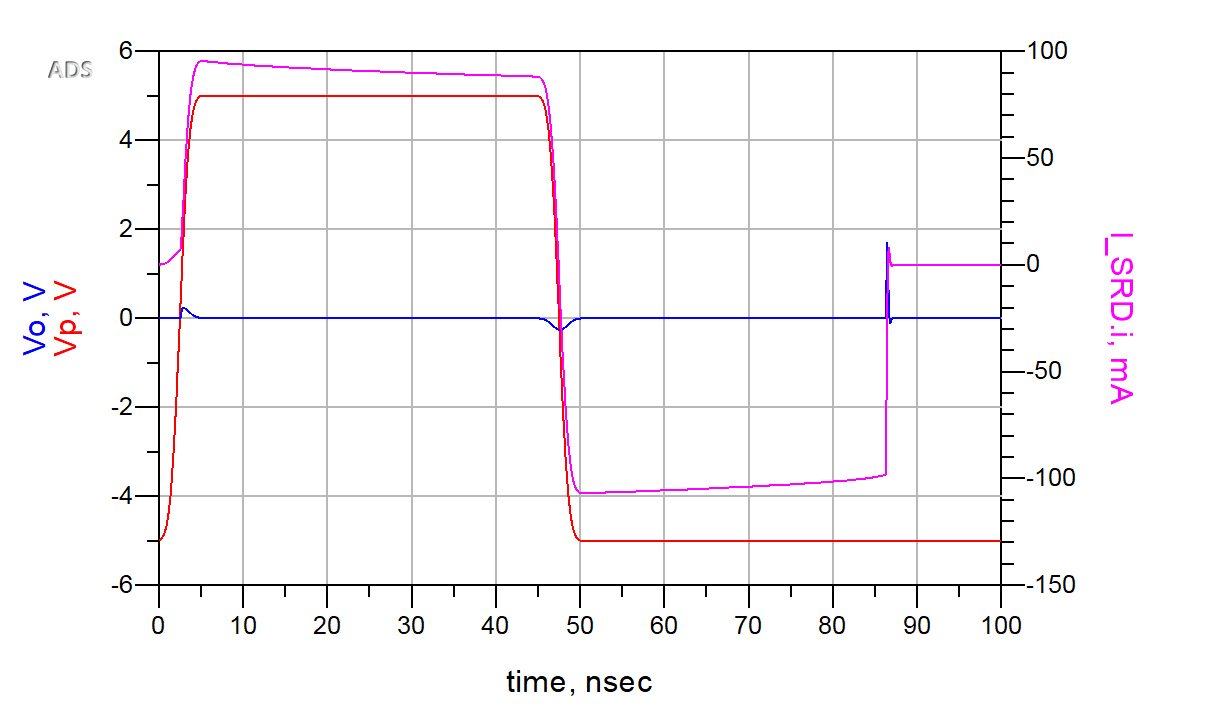
\includegraphics[width=0.8\textwidth]{images/stub_generator_result_waves.png}
    \caption{Resultado de simulación de generador con \textit{stub}}
    \label{fig:generator_result_waves}
\end{figure}

\begin{figure}[tbp]
    \centering
    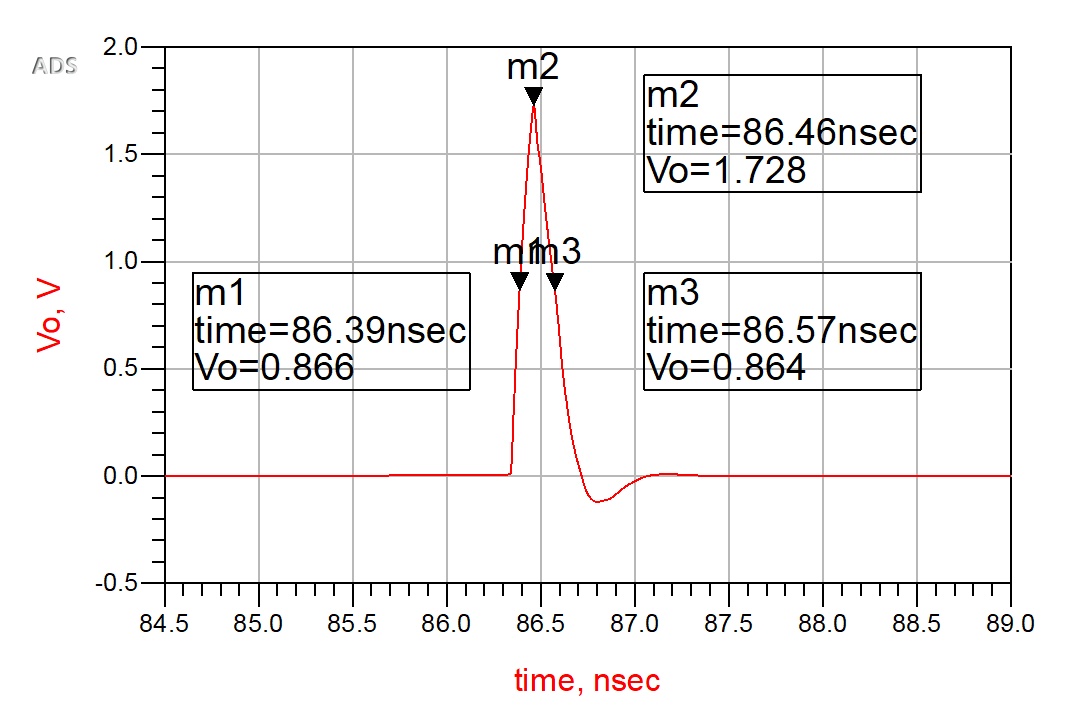
\includegraphics[width=0.8\textwidth]{images/stub_generator_result_pulse.png}
    \caption{Pulso simulado con generador con \textit{stub}}
    \label{fig:stub_generator_result_pulse}
\end{figure}

Vemos que el pulso tiene un ancho igual al doble del stub. vemos que se generan
pulsos espureos con los flancos de la señal de entrada. Vemos que se el pulso
final tiene un undershoot. vemos que la corriente baja abruptamente a 0. Vemos
que ahora la corriente es Vp/Rs, RL ya no entra en juego porque esta
cortocircuitada por el stub.

Hablar sobre la falta de reflexiones en el stub por ser de 50 ohm, q es la
impedancia q ve una vez q se abre el SRD? ver q pasa si movemos esa Zo?

\subsubsection{Calculo de stub}

En algún lado explicar cómo obtuvimos el largo en mm del stub.

\subsubsection{Diseño final del \textit{pulser}}

Incluir diodo \textit{Schottky}

\subsection{Diseño del \textit{driver}}

